\let\negmedspace\undefined
\let\negthickspace\undefined
\documentclass[journal,12pt,onecolumn]{IEEEtran}
\usepackage{cite}
\usepackage{amsmath,amssymb,amsfonts,amsthm}
\usepackage{algorithmic}
\usepackage{graphicx}
\graphicspath{{./figs/}}
\usepackage{textcomp}
\usepackage{xcolor}
\usepackage{txfonts}
\usepackage{listings}
\usepackage{enumitem}
\usepackage{mathtools}
\usepackage{gensymb}
\usepackage{comment}
\usepackage{caption}
\usepackage[breaklinks=true]{hyperref}
\usepackage{tkz-euclide} 
\usepackage{listings}
\usepackage{gvv}                                        
%\def\inputGnumericTable{}                                 
\usepackage[latin1]{inputenc}     
\usepackage{xparse}
\usepackage{color}                                            
\usepackage{array}                                            
\usepackage{longtable}                                       
\usepackage{calc}                                             
\usepackage{multirow}
\usepackage{multicol}
\usepackage{hhline}                                           
\usepackage{ifthen}                                           
\usepackage{lscape}\usepackage{tabularx}\usepackage{array}\usepackage{float}\usepackage{mhchem}\newtheorem{theorem}{Theorem}[section]
\newtheorem{problem}{Problem}
\newtheorem{proposition}{Proposition}[section]
\newtheorem{lemma}{Lemma}[section]
\newtheorem{corollary}[theorem]{Corollary}

\begin{document}
\title{ASSIGNMENT: GATE 2021 \\ CY: CHEMISTRY}
\author{EE25BTECH11039 - Manupati Manideep}
\date{Your Date Here}
\maketitle
\section*{Q.1 - Q.5 mcq, carry one mark each}
\begin{enumerate}
    \item Getting to the top is \_\_\_\_ than staying on top.
    \begin{multicols}{2}
    \begin{enumerate}
        \item more easy
        \item much easy
        \item easiest
        \item easier
    \end{enumerate}
    \end{multicols}
    \hfill{\brak{\text{GATE CY - 2021}}}

    \item The mirror image of the above text about the x-axis is: 
    \begin{center}
    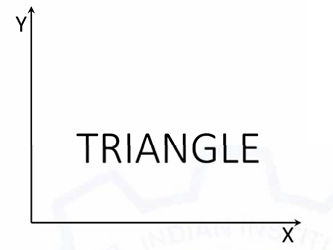
\includegraphics[width=0.4\columnwidth]{figs/q2.png}
    \end{center}
    \begin{multicols}{2}
    \begin{enumerate}
        \item 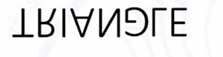
\includegraphics[width=0.4\columnwidth]{figs/q2a.png}
        \item 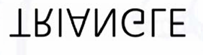
\includegraphics[width=0.4\columnwidth]{figs/q2b.png}
        \item 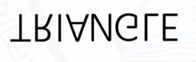
\includegraphics[width=0.4\columnwidth]{figs/q2c.png}
        \item 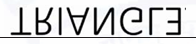
\includegraphics[width=0.4\columnwidth]{figs/q2d.png}
    \end{enumerate}
    \end{multicols}
    \hfill{\brak{\text{GATE CY - 2021}}}

    \item In a company, 35\% of the employees drink coffee, 40\% of the employees drink tea and 10\% of the employees drink both tea and coffee. What \% of employees drink neither tea nor coffee?
    \begin{multicols}{2}
    \begin{enumerate}
        \item 15
        \item 25
        \item 35
        \item 40
    \end{enumerate}
    \end{multicols}
    \hfill{\brak{\text{GATE CY - 2021}}}

    \item $\oplus$ and $\odot$ are two operators on numbers p and q such that $p\oplus q=\frac{p^{2}+q^{2}}{pq}$ and $p\odot q=\frac{p^{2}}{q};$ If $x\oplus y=2\odot2$ then $x=$
    \begin{multicols}{2}
    \begin{enumerate}
        \item $\frac{y}{2}$
        \item y
        \item $\frac{3y}{2}$
        \item 2 y
    \end{enumerate}
    \end{multicols}
    \hfill{\brak{\text{GATE CY - 2021}}}
    
    \item Four persons P, Q, R and S are to be seated in a row, all facing the same direction, but not necessarily in the same order. P and R cannot sit adjacent to each other. S should be seated to the right of Q. The number of distinct seating arrangements possible is:
    \begin{multicols}{2}
    \begin{enumerate}
        \item 2
        \item 4
        \item 6
        \item 8
    \end{enumerate}
    \end{multicols}
    \hfill{\brak{\text{GATE CY - 2021}}}
\section*{Q.6 - Q.10 mcq, carry two marks each} 
    \item Statement: Either P marries Q or X marries Y. Among the options below, the logical NEGATION of the above statement is:
    \begin{multicols}{2}
    \begin{enumerate}
        \item P does not marry Q and X marries Y.
        \item Neither P marries Q nor X marries Y.
        \item X does not marry Y and P marries Q.
        \item P marries Q and X marries Y.
    \end{enumerate}
    \end{multicols}
    \hfill{\brak{\text{GATE CY - 2021}}}

    \item Consider two rectangular sheets, Sheet M and Sheet N of dimensions 6 cm x 4 cm each. Folding operation 1: The sheet is folded into half by joining the short edges of the current shape. Folding operation 2: The sheet is folded into half by joining the long edges of the current shape. Folding operation 1 is carried out on Sheet M three times. Folding operation 2 is carried out on Sheet N three times. The ratio of perimeters of the final folded shape of Sheet N to the final folded shape of Sheet M is:
    \begin{multicols}{2}
    \begin{enumerate}
        \item 13:7
        \item 3:2
        \item 7:5
        \item 5:13
    \end{enumerate}
    \end{multicols}
    \hfill{\brak{\text{GATE CY - 2021}}}
    
    \item Five line segments of equal lengths, PR, PS, QS, QT and RT are used to form a star as shown in the figure above. The value of $\theta$, in degrees, is: 
    \begin{center}
    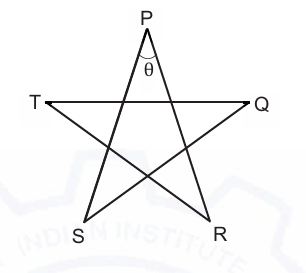
\includegraphics[width=0.4\columnwidth]{figs/q8.png}
    \end{center}
    \begin{multicols}{2}
    \begin{enumerate}
        \item 36
        \item 45
        \item 72
        \item 108
    \end{enumerate}
    \end{multicols}
    \hfill{\brak{\text{GATE CY - 2021}}}

    \item A function, $\lambda$, is defined by $\lambda\brak{p,q}=\begin{cases}\brak{p-q}^{2},&if~p\ge q,\\ p+q,&if~p<q.\end{cases}$ The value of the expression $\frac{\lambda\brak{-\brak{-3+2},\brak{-2+3}}}{\brak{-\brak{-2+1}}}$ is:
    \begin{multicols}{2}
    \begin{enumerate}
        \item -1
        \item 0
        \item $\frac{16}{3}$
        \item 16
    \end{enumerate}
    \end{multicols}
    \hfill{\brak{\text{GATE CY - 2021}}}

    \item Humans have the ability to construct worlds entirely in their minds, which don't exist in the physical world. So far as we know, no other species possesses this ability. This skill is so important that we have different words to refer to its different flavors, such as imagination, invention and innovation. Based on the above passage, which one of the following is TRUE?
    
    \begin{enumerate}
        \item No species possess the ability to construct worlds in their minds.
        \item The terms imagination, invention and innovation refer to unrelated skills.
        \item We do not know of any species other than humans who possess the ability to construct mental worlds.
        \item Imagination, invention and innovation are unrelated to the ability to construct mental worlds.
    \end{enumerate}
    
    \hfill{\brak{\text{GATE CY - 2021}}}
\section*{Q.11 - Q.24 carry one mark each}    
 \item The rates of alkaline hydrolysis of the compounds shown below follow the order: 
    \begin{center}
    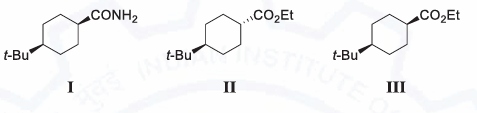
\includegraphics[width=0.8\columnwidth]{figs/q11.png}
    \end{center}
    \begin{multicols}{2}
    \begin{enumerate}
        \item I $>$ II $>$ III
        \item II $>$ I $>$ III
        \item II $>$ III $>$ I
        \item III $>$ I $>$ II
    \end{enumerate}
    \end{multicols}
    \hfill{\brak{\text{GATE CY-2021}}}

    \item The major product formed in the following reaction is: 
    \begin{center}
    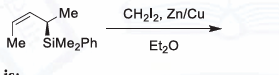
\includegraphics[width=0.4\columnwidth]{figs/q12.png}
    \end{center}
    \begin{multicols}{2}
    \begin{enumerate}
        \item 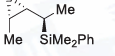
\includegraphics[width=0.4\columnwidth]{figs/q12a.png}
        \item 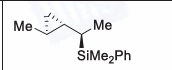
\includegraphics[width=0.4\columnwidth]{figs/q12b.png}
        \item 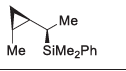
\includegraphics[width=0.4\columnwidth]{figs/q12c.png}
        \item 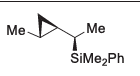
\includegraphics[width=0.4\columnwidth]{figs/q12d.png}
    \end{enumerate}
    \end{multicols}
    \hfill{\brak{\text{GATE CY-2021}}}

    \item The major product formed in the following reaction is: 
    \begin{center}
    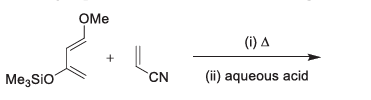
\includegraphics[width=0.8\columnwidth]{figs/q13.png}
    \end{center}
    \begin{multicols}{2}
    \begin{enumerate}
        \item 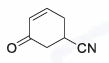
\includegraphics[width=0.4\columnwidth]{figs/q13a.png}
        \item 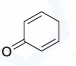
\includegraphics[width=0.4\columnwidth]{figs/q13b.png}
        \item 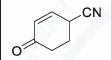
\includegraphics[width=0.4\columnwidth]{figs/q13c.png}
        \item 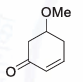
\includegraphics[width=0.4\columnwidth]{figs/q13d.png}
    \end{enumerate}
    \end{multicols}
    \hfill{\brak{\text{GATE CY-2021}}}

    \item The least acidic among the following compounds is: 
    \begin{center}
    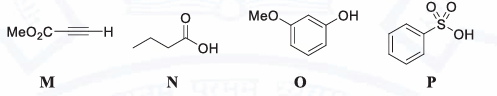
\includegraphics[width=0.8\columnwidth]{figs/q14.png}
    \end{center}
    \begin{multicols}{2}
    \begin{enumerate}
        \item M
        \item N
        \item O
        \item P
    \end{enumerate}
    \end{multicols}
    \hfill{\brak{\text{GATE CY-2021}}}
    
    \item The major product formed in the following reaction is: 
    \begin{center}
    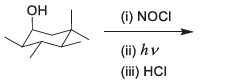
\includegraphics[width=0.6\columnwidth]{figs/q15.png}
    \end{center}
    \begin{multicols}{2}
    \begin{enumerate}
        \item 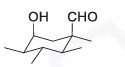
\includegraphics[width=0.4\columnwidth]{figs/q15a.png}
        \item 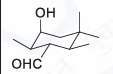
\includegraphics[width=0.4\columnwidth]{figs/q15b.png}
        \item 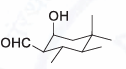
\includegraphics[width=0.4\columnwidth]{figs/q15c.png}
        \item 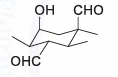
\includegraphics[width=0.4\columnwidth]{figs/q15d.png}
    \end{enumerate}
    \end{multicols}
    \hfill{\brak{\text{GATE CY-2021}}}

    \item The reagent\brak{s} required for the conversion of hex-3-yne to \brak{E}-hex-3-ene is/are:
    \begin{multicols}{2}
    \begin{enumerate}
        \item H2, $Pd/BaSO_{4}$
        \item Bu3SnH
        \item Li/liquid NH3
        \item LiAlH4
    \end{enumerate}
    \end{multicols}
    \hfill{\brak{\text{GATE CY-2021}}}

    \item An organic compound exhibits the $\sbrak{M}^+$, $\sbrak{M+2}^-$ and $\sbrak{M+4}^-$ peaks in the intensity ratio 1:2:1 in the mass spectrum, and shows a singlet at $\delta$ 7.49 in the $^1$H NMR spectrum in $CDCl_3$. The compound is:
    \begin{multicols}{2}
    \begin{enumerate}
        \item 1,4-dichlorobenzene
        \item 1,4-dibromobenzene
        \item 1,2-dibromobenzene
        \item 1,2-dichlorobenzene
    \end{enumerate}
    \end{multicols}
    \hfill{\brak{\text{GATE CY-2021}}}
    
    \item Reaction of $LiAlH_4$ with one equivalent of $Me_3N \cdot HCl$ gives a tetrahedral compound, which reacts with another equivalent of $Me_3N \cdot HCl$ to give compound N. The compound N and its geometry, respectively, are:
    \begin{multicols}{2}
    \begin{enumerate}
        \item $LiAlH_4NMe_3$ and trigonal bipyramidal
        \item $Li_2AlH_4Cl$ and square pyramidal
        \item $AlH_3\brak{NMe_3}_2$ and trigonal bipyramidal
        \item $AlH_3\brak{NMe_3}_2$ and pentagonal
    \end{enumerate}
    \end{multicols}
    \hfill{\brak{\text{GATE CY-2021}}}

    \item Which one of the following is a non-heme protein?
    \begin{multicols}{2}
    \begin{enumerate}
        \item hemoglobin
        \item hemocyanin
        \item myoglobin
        \item cytochrome P-450
    \end{enumerate}
    \end{multicols}
    \hfill{\brak{\text{GATE CY-2021}}}
    
    \item A correct example of a nucleotide is:
    \begin{multicols}{2}
    \begin{enumerate}
        \item adenosine monophosphate \brak{AMP}
        \item RNA
        \item uridine
        \item DNA
    \end{enumerate}
    \end{multicols}
    \hfill{\brak{\text{GATE CY-2021}}}
     \item The equilibrium constant for the reaction
    \begin{center}
        3 NO \brak{g} $\rightleftharpoons$ N$_2$O \brak{g} + NO$_2$ \brak{g}
    \end{center}
    at 25 $\degree$C is closest to: [$\Delta$G$\degree$ = -104.18 kJ; R = 8.314 J mol$^{-1}$ K$^{-1}$]
    \begin{multicols}{2}
    \begin{enumerate}
        \item 1.043
        \item 1.8 $\times$ 10$^{18}$
        \item 1.651
        \item 5.7 $\times$ 10$^{-19}$
    \end{enumerate}
    \end{multicols}
    \hfill{\brak{\text{GATE CY-2021}}}

    \item The reaction of NiBr$_{2}$ with two equivalents of PPh$_{3}$ in CS$_{2}$ at -78 $\degree$C gives a red-colored diamagnetic complex, [NiBr$_{2}$\brak{PPh_{3}}$_{2}$]. This transforms to a green-colored paramagnetic complex with the same molecular formula at 25 $\degree$C. The geometry and the number of unpaired electrons in the green-colored complex, respectively, are:
    \begin{multicols}{2}
    \begin{enumerate}
        \item tetrahedral and 1
        \item tetrahedral and 2
        \item square planar and 2
        \item square planar and 4
    \end{enumerate}
    \end{multicols}
    \hfill{\brak{\text{GATE CY-2021}}}

    \item The rate of the substitution reaction of [Co\brak{CN}$_{5}$Cl]$^{3-}$ with OH$^{-}$ to give [Co\brak{CN}$_{5}$\brak{OH}]$^{3-}$
    \begin{multicols}{2}
    \begin{enumerate}
        \item depends on the concentrations of both [Co\brak{CN}$_{5}$Cl]$^{3-}$ and OH$^{-}$
        \item depends on the concentration of [Co\brak{CN}$_{5}$Cl]$^{3-}$ only
        \item is directly proportional to the concentration of OH$^{-}$ only
        \item is inversely proportional to the concentration of OH$^{-}$
    \end{enumerate}
    \end{multicols}
    \hfill{\brak{\text{GATE CY-2021}}}

    \item The $\Delta_o$ of [Cr\brak{H_2O}$_6$]$^{3+}$, [CrF$_6$]$^{3-}$ and [Cr\brak{CN}$_6$]$^{3-}$ follows the order:
    
    \begin{enumerate}
        \item$[Cr\brak{H_2O}_6]^{3+} > [CrF_6]^{3-} > [Cr\brak{CN}_6]^{3-}$
        \item $[CrF_6]^{3-} > [Cr\brak{H_2O}_6]^{3+} > [Cr\brak{CN}_6]^{3-}$
        \item $[Cr\brak{CN}_6]^{3-} > [Cr\brak{H_2O}_6]^{3+} > [CrF_6]^{3-}$
        \item$[CrF_6]^{3-} > [Cr\brak{CN}_6]^{3-} > [Cr\brak{H_2O}_6]^{3+}$
    \end{enumerate}
   
    \hfill{\brak{\text{GATE CY-2021}}}
\section*{Q.25 - Q.28 multiple select question, carry one mark each}

    \item The phase diagram of CO$_2$ is shown below:
    \begin{center}
    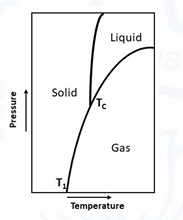
\includegraphics[width=0.4\columnwidth]{figs/q25.png}
    \end{center}
    The correct statement\brak{s} about CO$_2$ is/are:
    \begin{multicols}{2}
    \begin{enumerate}
        \item Below T$_c$, it does not exist in liquid state.
        \item Above T$_c$, it does not exist in liquid state.
        \item At T$_c$, it can exist in all three phases.
        \item Above T$_2$, it does not exist in solid state.
    \end{enumerate}
    \end{multicols}
    \hfill{\brak{\text{GATE CY-2021}}}

    \item Acceptable wavefunctions for a quantum particle must be:
    \begin{multicols}{2}
    \begin{enumerate}
        \item odd
        \item even
        \item single-valued
        \item continuous
    \end{enumerate}
    \end{multicols}
    \hfill{\brak{\text{GATE CY-2021}}}

    \item The characters of E, C$_2$, $\sigma_v$, and $\sigma'_v$ symmetry operations, in this order, for valid irreducible representation\brak{s} of the C$_{2v}$ point group is/are:
    \begin{multicols}{2}
    \begin{enumerate}
        \item 1, 1, 1, 1
        \item 1, 1, -1, -1
        \item 1, -1, 1, -1
        \item 1, -1, -1, 1
    \end{enumerate}
    \end{multicols}
    \hfill{\brak{\text{GATE CY-2021}}}

    \item The normal mode\brak{s} of vibration of H$_2$O is/are:
    
    \begin{enumerate}
        \item 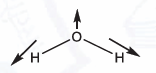
\includegraphics[width=0.25\columnwidth]{figs/q28a.png}
        \item 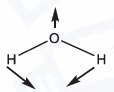
\includegraphics[width=0.25\columnwidth]{figs/q28b.png}
        \item 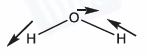
\includegraphics[width=0.25\columnwidth]{figs/q28c.png}
        \item 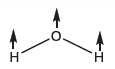
\includegraphics[width=0.25\columnwidth]{figs/q28d.png}
    \end{enumerate}
    
    \hfill{\brak{\text{GATE CY-2021}}}
\section*{Q.29 - Q.35 numerical answer type, carry one mark each}

    \item A reversible heat engine absorbs 20 kJ of heat from a source at 500 K and dissipates it to the reservoir at 400 K. The efficiency of the heat engine is \_\_\_\_\_\_\_\_ \%.
    \hfill{\brak{\text{GATE CY-2021}}}

    \item Among the following eight compounds, the number of compound\brak{s} which can exhibit stereoisomerism is \_\_\_\_\_\_\_.
    \begin{center}
    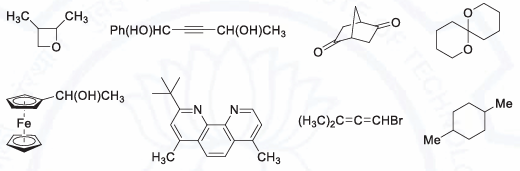
\includegraphics[width=0.8\columnwidth]{figs/q30.png}
    \end{center}
    \hfill{\brak{\text{GATE CY-2021}}}
 \item The Mo-Mo bond order in [\brak{K_5-C_5H_5}Mo\brak{CO}$_2$]$_2$ which obeys the 18-electron rule is \_\_\_\_\_\_\_.
    \hfill{\brak{\text{GATE CY-2021}}}

    \item The change in enthalpy \brak{\Delta H} for the reaction
    \begin{center}
        2 P \brak{s} +  Br$_2$ \brak{l} $\rightarrow$ 2 PBr$_3$ \brak{l}
    \end{center}
    is -243 kJ. In this reaction, if the amount of phosphorus consumed is 3.1 g, the change in enthalpy \brak{\text{rounded off to two decimal places}} is \_\_\_\_\_\_\_\_ kJ. [Atomic Wt. of P = 31]
    \hfill{\brak{\text{GATE CY-2021}}}

    \item The number of signal\brak{s} in the $^1$H NMR spectrum of the following compound recorded at 25 $\degree$C in CDCl$_3$ is \_\_\_\_\_\_\_.
    \begin{center}
    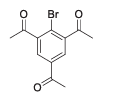
\includegraphics[width=0.25\columnwidth]{figs/q33.png}
    \end{center}
    \hfill{\brak{\text{GATE CY-2021}}}

    \item A 5 V battery delivers a steady current of 1.5 A for a period of 2 h. The total charge that has passed through the circuit is \_\_\_\_\_\_\_\_ Coulombs.
    \hfill{\brak{\text{GATE CY-2021}}}

    \item The spin-only magnetic moment of [Co\brak{H_2O}$_6$]$^{2+}$ \brak{\text{rounded off to one decimal place}} is \_\_\_\_\_\_\_\_ BM.
    \hfill{\brak{\text{GATE CY-2021}}}
\section*{Q.36 - Q.52 mcq, carry two mark each}

    \item The geometry and the number of unpaired electrons in tetrakis\brak{1-norbornyl}Co, respectively, are:
    \begin{multicols}{2}
    \begin{enumerate}
        \item tetrahedral and one
        \item tetrahedral and five
        \item square planar and one
        \item square planar and three
    \end{enumerate}
    \end{multicols}
    \hfill{\brak{\text{GATE CY-2021}}}

    \item The yellow color of an aqueous solution of K$_2$CrO$_4$ changes to red-orange upon the addition of a few drops of HCl. The red-orange complex, the oxidation state of its central element\brak{s}, and the origin of its color, respectively, are:
    \begin{multicols}{2}
    \begin{enumerate}
        \item chromium chloride, +3, d-d transition
        \item dichromate ion, +6 and +6, charge transfer
        \item perchlorate ion, +7, charge transfer
        \item chromic acid, +6, charge transfer
    \end{enumerate}
    \end{multicols}
    \hfill{\brak{\text{GATE CY-2021}}}

    \item The shapes of the compounds ClF$_3$, XeOF$_2$, N$_3^-$ and XeO$_3$F$_2$ respectively, are:
    \begin{multicols}{2}
    \begin{enumerate}
        \item T-shape, T-shape, linear and trigonal bipyramidal
        \item trigonal planar, T-shape, V-shape and square pyramidal
        \item T-shape, trigonal planar, linear and square pyramidal
        \item trigonal planar, trigonal planar, V-shape and trigonal bipyramidal
    \end{enumerate}
    \end{multicols}
    \hfill{\brak{\text{GATE CY-2021}}}

    \item The metal borides that contain isolated boron atoms are:
    \begin{multicols}{2}
    \begin{enumerate}
        \item Tc$_7$B$_3$ and Re$_7$B$_3$
        \item Cr$_5$B$_3$ and V$_3$B$_2$
        \item Ti$_4$B$_4$ and V$_3$B$_4$
        \item TiB and HfB
    \end{enumerate}
    \end{multicols}
    \hfill{\brak{\text{GATE CY-2021}}}

    \item The major product formed in the following reaction is:
    \begin{center}
    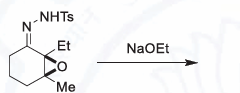
\includegraphics[width=0.4\columnwidth]{figs/q40.png}
    \end{center}
    \begin{multicols}{2}
    \begin{enumerate}
        \item non-6-yn-2-one
        \item non-3-yn-8-one
        \item non-2-yn-6-one
        \item non-3-en-8-one
    \end{enumerate}
    \end{multicols}
    \hfill{\brak{\text{GATE CY-2021}}}
 \item The major product formed in the following reaction 
    \begin{center}
    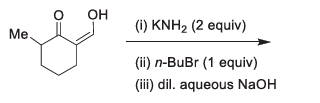
\includegraphics[width=0.4\columnwidth]{figs/q41.png}
    \end{center}
    is:
    \begin{multicols}{2}
    \begin{enumerate}
        \item 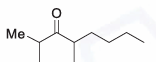
\includegraphics[width=0.4\columnwidth]{figs/q41a.png}
        \item 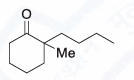
\includegraphics[width=0.4\columnwidth]{figs/q41b.png}
        \item 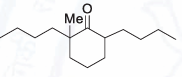
\includegraphics[width=0.4\columnwidth]{figs/q41c.png}
        \item 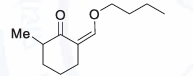
\includegraphics[width=0.4\columnwidth]{figs/q41d.png}
    \end{enumerate}
    \end{multicols}
    \hfill{\brak{\text{GATE CY-2021}}}

    \item The major product formed in the following reaction 
    \begin{center}
    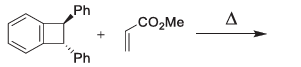
\includegraphics[width=0.4\columnwidth]{figs/q42.png}
    \end{center}
    is:
    \begin{multicols}{2}
    \begin{enumerate}
        \item 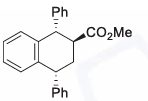
\includegraphics[width=0.4\columnwidth]{figs/q42a.png}
        \item 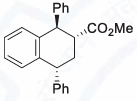
\includegraphics[width=0.4\columnwidth]{figs/q42b.png}
        \item 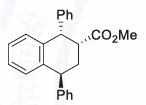
\includegraphics[width=0.4\columnwidth]{figs/q42c.png}
        \item 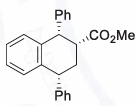
\includegraphics[width=0.4\columnwidth]{figs/q42d.png}
    \end{enumerate}
    \end{multicols}
    \hfill{\brak{\text{GATE CY-2021}}}
    
    \item In the following reaction sequence the major products P and Q, respectively, are:
    \begin{center}
    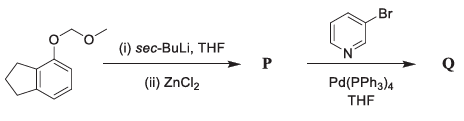
\includegraphics[width=0.8\columnwidth]{figs/q43.png}
    \end{center}
    
    \begin{enumerate}
        \item 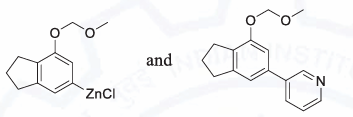
\includegraphics[width=0.25\columnwidth]{figs/q43a.png}
        \item 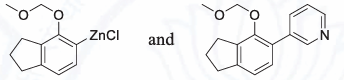
\includegraphics[width=0.25\columnwidth]{figs/q43b.png}
        \item 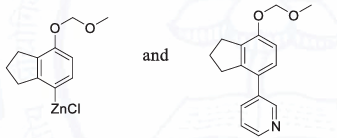
\includegraphics[width=0.25\columnwidth]{figs/q43c.png}
        \item 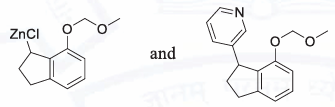
\includegraphics[width=0.25\columnwidth]{figs/q43d.png}
    \end{enumerate}
    \hfill{\brak{\text{GATE CY-2021}}}

    \item In an electrochemical cell, Ag$^+$ ions in AgNO$_3$ are reduced to Ag metal at the cathode and Cu is oxidized to Cu$^{2+}$ at the anode. A current of 0.7 A is passed through the cell for 10 min. The mass \brak{\text{in grams}} of silver deposited and copper dissolved, respectively, are: \sbrak{Faraday Constant = 96,485 C mol^{-1}, Atomic Weight of Ag = 107.9, Atomic Weight of Cu = 63.55}
    \begin{multicols}{2}
    \begin{enumerate}
        \item 0.469 and 0.138
        \item 0.235 and 0.138
        \item 0.469 and 0.069
        \item 0.235 and 0.069
    \end{enumerate}
    \end{multicols}
    \hfill{\brak{\text{GATE CY-2021}}}
    
    \item Among the following the compounds which can be prepared by nucleophilic substitution reaction are:
    \begin{center}
    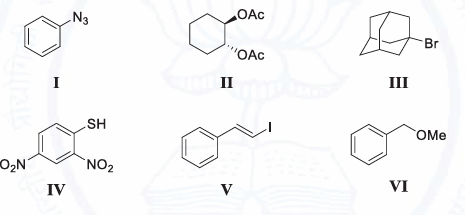
\includegraphics[width=0.8\columnwidth]{figs/q45.png}
    \end{center}
    \begin{multicols}{2}
    \begin{enumerate}
        \item III, IV, and V
        \item I, II, and VI
        \item II, IV, and VI
        \item I, III, and V
    \end{enumerate}
    \end{multicols}
    \hfill{\brak{\text{GATE CY-2021}}}

    \item In the following reaction
    \begin{center}
    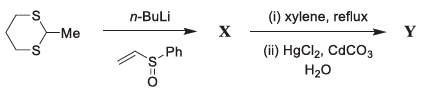
\includegraphics[width=0.8\columnwidth]{figs/q46.png}
    \end{center}
    the major products X and Y, respectively, are:

    \begin{enumerate}
        \item 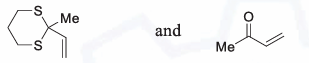
\includegraphics[width=0.4\columnwidth]{figs/q46a.png}
        \item 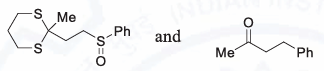
\includegraphics[width=0.4\columnwidth]{figs/q46b.png}
        \item \includegraphics[width=0.4\columnwidth]{figs/q46c.png}
        \item \includegraphics[width=0.4\columnwidth]{figs/q46d.png}
    \end{enumerate}
    
    \hfill{\brak{\text{GATE CY-2021}}}
    
    \item The major products P and Q formed in the following reactions respectively, are:
    \begin{center}
    \includegraphics[width=0.8\columnwidth]{figs/q47.png}
    \end{center}
    
    \begin{enumerate}
        \item \includegraphics[width=0.25\columnwidth]{figs/q47a.png}
        \item \includegraphics[width=0.25\columnwidth]{figs/q47b.png}
        \item \includegraphics[width=0.25\columnwidth]{figs/q47c.png}
        \item \includegraphics[width=0.25\columnwidth]{figs/q47d.png}
    \end{enumerate}
    \hfill{\brak{\text{GATE CY-2021}}}

    \item The major product formed in the reaction of \brak{2R,3R}-2-bromo-3-methylpentane with NaOMe is:
    \begin{multicols}{2}
    \begin{enumerate}
        \item \brak{Z}-3-methylpent-2-ene
        \item \brak{E}-3-methylpent-2-ene
        \item \brak{2R,3R}-2-methoxy-3-methylpentane
        \item \brak{2S,3R}-2-methoxy-3-methylpentane
    \end{enumerate}
    \end{multicols}
    \hfill{\brak{\text{GATE CY-2021}}}

    \item The major product formed in the following reaction is:
    \begin{center}
    \includegraphics[width=0.8\columnwidth]{figs/q49.png}
    \end{center}
    \begin{multicols}{2}
    \begin{enumerate}
        \item \includegraphics[width=0.4\columnwidth]{figs/q49a.png}
        \item \includegraphics[width=0.4\columnwidth]{figs/q49b.png}
        \item \includegraphics[width=0.4\columnwidth]{figs/q49c.png}
        \item \includegraphics[width=0.4\columnwidth]{figs/q49d.png}
    \end{enumerate}
    \end{multicols}
    \hfill{\brak{\text{GATE CY-2021}}}

    \item Hexane and heptane are completely miscible. At 25 $\degree$C, the vapor pressures of hexane and heptane are 0.198 atm and 0.06 atm, respectively. The mole fractions of hexane and heptane in the vapor phase for a solution containing 4 M hexane and 6 M heptane, respectively, are:
    \begin{multicols}{2}
    \begin{enumerate}
        \item 0.688 and 0.312
        \item 0.400 and 0.600
        \item 0.312 and 0.688
        \item 0.600 and 0.400
    \end{enumerate}
    \end{multicols}
    \hfill{\brak{\text{GATE CY-2021}}}
  \item The correct order of Lewis acid strengths of BF$_2$Cl, BFClBr, BF$_2$Br and BFBr$_2$ is:
    \begin{multicols}{2}
    \begin{enumerate}
        \item BF$_2$Cl $>$ BFClBr $>$ BF$_2$Br $>$ BFBr$_2$
        \item BFBr$_2$ $>$ BFClBr $>$ BF$_2$Br $>$ BF$_2$Cl
        \item BF$_2$Cl $>$ BF$_2$Br $>$ BFClBr $>$ BFBr$_2$
        \item BFClBr $>$ BFBr$_2$ $>$ BF$_2$Cl $>$ BF$_2$Br
    \end{enumerate}
    \end{multicols}
    \hfill{\brak{\text{GATE CY-2021}}}

    \item The correct order of increasing intensity \brak{\text{molar absorptivity}} of the UV-visible absorption bands for the ions [Ti\brak{H_2O}$_6$]$^{3+}$, [Mn\brak{H_2O}$_6$]$^{2+}$, [CrO$_4$]$^{2-}$, and [NiCl$_4$]$^{2-}$ is:
    
 \begin{enumerate}
    \item $[Ti\brak{H_2O}_6]^{3+}$ $<$ $[Mn\brak{H_2O}_6]^{2+}$ $<$ $[CrO_4]^{2-}$
    \item $[Mn\brak{H_2O}_6]^{2+}$ $<$ $[Ti\brak{H_2O}_6]^{3+}$ $<$ $[CrO_4]^{2-}$
    \item $[NiCl_4]^{2-}$ $<$ $[Ti\brak{H_2O}_6]^{3+}$ $<$ $[Mn\brak{H_2O}_6]^{2+}$
    \item $[NiCl_4]^{2-}$ $<$ $[Mn\brak{H_2O}_6]^{2+}$ $<$ $[Ti\brak{H_2O}_6]^{3+}$
\end{enumerate}
    
    \hfill{\brak{\text{GATE CY-2021}}}

    \item The correct statement\brak{s} about the concentration of Na$^+$ and K$^+$ ions in animal cells is/are:
   
    \begin{enumerate}
       
 \item$[Na^+] \text{inside the cell} > [Na^+] \text{outside the cell}$
 \item$[K^+] inside the cell > [K^+] outside the cell$
 \item$[Na^+] inside the cell < [Na^+] outside the cell$
 \item$[K^+] inside the cell < [K^+] outside the cell$
    \end{enumerate}
    
    \hfill{\brak{\text{GATE CY-2021}}}

    \item The correct statement\brak{s} about actinides is/are:
    
    \begin{enumerate}
        \item The 5f electrons of actinides are bound less tightly than the 4f electrons.
        \item The trans uranium elements are prepared artificially.
        \item All the actinides are radioactive.
        \item Actinides do not exhibit actinide contraction.
    \end{enumerate}
    
    \hfill{\brak{\text{GATE CY-2021}}}
\section*{Q.55 - Q.65 numerical answer type, carry two mark each}

    \item The number of photons emitted per nanosecond by a deuterium lamp \brak{400 nm} having a power of 1 microwatt \brak{\text{rounded off to the nearest integer}} is \_\_\_\_\_\_\_. [h = 6.626 $\times$ 10$^{-34}$ kg m$^2$ s$^{-1}$; c = 3.0 $\times$ 10$^8$ m s$^{-1}$]
    \hfill{\brak{\text{GATE CY-2021}}}

    \item Given the initial weight of 1 mg of radioactive $^{106}Ru$ \brak{\text{half-life = 5.27 years}}, the amount disintegrated in 1 year \brak{\text{rounded off to two decimal places}} is \_\_\_\_\_\_\_ mg.
    \hfill{\brak{\text{GATE CY-2021}}}

    \item The de Broglie wavelength of an argon atom \brak{mass = 40 amu} traveling at a speed of 250 m s$^{-1}$ \brak{\text{rounded off to one decimal place}} is \_\_\_\_\_\_\_\_ picometers. [N = 6.022 $\times$ 10$^{23}$; h = 6.626 $\times$ 10$^{-34}$ kg m$^2$ s$^{-1}$]
    \hfill{\brak{\text{GATE CY-2021}}}
    
    \item The molar absorption coefficient of a substance dissolved in cyclohexane is 1710 L mol$^{-1}$ cm$^{-1}$ at 500 nm. The reduction in intensity of light of the same wavelength that passes through a cell of 1 mm path length containing a 2 mmol L$^{-1}$ solution \brak{\text{rounded off to one decimal place}} is \_\_\_\_\_\_\_\_ \%.
    \hfill{\brak{\text{GATE CY-2021}}}

    \item The fundamental vibrational frequency of $^1H^{127}I$ is 2309 cm$^{-1}$. The force constant for this molecule \brak{\text{rounded off to the nearest integer}} is \_\_\_\_\_\_\_\_ N m$^{-1}$. [N = 6.022 $\times$ 10$^{23}$, c = 3.0 $\times$ 10$^8$ m s$^{-1}$]
    \hfill{\brak{\text{GATE CY-2021}}}

    \item A laser Raman spectrometer operating at 532 nm is used to record the vibrational spectrum of Cl$_2$ having its fundamental vibration at 560 cm$^{-1}$. The Stokes line corresponding to this vibration will be observed at \_\_\_\_\_\_\_\_ cm$^{-1}$. \brak{\text{Rounded off to the nearest integer}}
    \hfill{\brak{\text{GATE CY-2021}}}
\item The vapor pressure of toluene \brak{Mol. Wt. = 92} is 0.13 atm at 25 $^\circ$C. 
If 6 g of a hydrocarbon is dissolved in 92 g of toluene, the vapor pressure drops to 0.12 atm. 
The molar mass of the hydrocarbon \brak{\text{rounded off to the nearest integer}} is \_\_\_\_\_\_.
\hfill{\brak{\text{GATE CY-2021}}}


\item The reaction \\
CO \brak{g} + Cl$_2$ \brak{g} $\rightleftharpoons$ COCl$_2$ \brak{g} \\
at 500 $^\circ$C, with initial pressures of 0.7 bar of CO and 1.0 bar of Cl$_2$, is allowed to reach equilibrium. 
The partial pressure of COCl$_2$ \brak{g} at equilibrium is 0.15 bar. 
The equilibrium constant for this reaction at 500 $^\circ$C \brak{\text{rounded off to two decimal places}} is \_\_\_\_\_\_.
\hfill{\brak{\text{GATE CY-2021}}}

\item The rate constants for the decomposition of a molecule in the presence of oxygen are 
0.237 $\times$ 10$^{-4}$ L mol$^{-1}$ s$^{-1}$ at 0 $^\circ$C and 
2.64 $\times$ 10$^{-4}$ L mol$^{-1}$ s$^{-1}$ at 25 $^\circ$C 
\brak{R = 8.314 J mol^{-1} K^{-1}}. \\
The activation energy for this reaction \brak{\text{rounded off to one decimal place}} is \_\_\_\_\_\_ kJ mol$^{-1}$.
\hfill{\brak{\text{GATE CY-2021}}}


\item 2 L of a gas at 1 atm pressure is reversibly heated to reach a final volume of 3.5 L. 
The absolute value of the work done on the gas \brak{\text{rounded off to the nearest integer}} is \_\_\_\_\_\_ Joules.
\newline
\hfill{\brak{\text{GATE CY-2021}}}

\item The quantity of the cobalt ore [Co$_3$\brak{AsO_4}$_2 \cdot$H$_2$O] required to obtain 1 kg of cobalt \brak{\text{rounded off to two decimal places}} is \_\_\_\_\_\_ kg. \\

\hfill{\brak{\text{GATE CY-2021}}}

\begin{center}
    
\textbf{END OF THE QUESTION PAPER}
\end{center}    
\end{enumerate}
\end{document}
